%%%%%%%%%%%%%%%%%%%%%%%%%%%%%% LyX specific LaTeX commands.
%% Bold symbol macro for standard LaTeX users
\providecommand{\boldsymbol}[1]{\mbox{\boldmath $#1$}}

%% Because html converters don't know tabularnewline
\providecommand{\tabularnewline}{\\}

The chapter describes the usage of mathematical expressions for post
processing simulation data in ``Qucs'', how to enter formulas and
modifying them.  It gives a brief description of the overall syntax of
those expressions.

\tutsubsection{Entering Measurement Expressions}

Measurement expressions generate new datasets by function or operator
driven evaluation of simulation results. Those new datasets are
accessible in the data display tab after simulation. The related
equations can be entered into the schematic editor by the following
means:

\begin{itemize}
\item Using the equation icon in the {}``Tools'' bar (see fig. \ref{cap:Entering})
\item Using menu item {}``Insert'' $\rightarrow$ ''Insert equation''
\end{itemize}
%
\begin{figure}[ht]
\begin{center}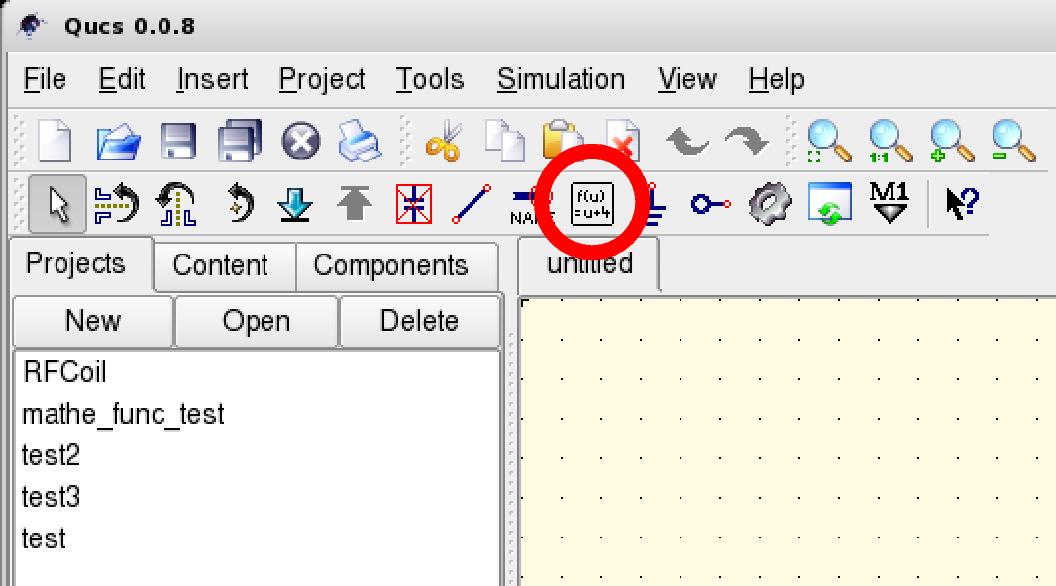
\includegraphics[%
  scale=0.4]{qucs_formula1}\end{center}


\caption{\label{cap:Entering}Entering a new measurement expression via equation
icon}
\end{figure}


You can now place the equation symbol by mouse click anywhere
in the schematic. Each mouse click creates a new equation instance
each consisting of a variable number of measurement expressions.
Press the <ESC> key if you do not like further equations.

Another option is to select an existing equation, copy it (either
by menu item {}``Edit'' $\rightarrow$ ''Copy'' or by <CTRL>+C%
\footnote{<CTRL>+C means that you have to press the <CTRL> key and the C key
simultaneously.%
}) and paste it (either by menu item {}``Edit'' $\rightarrow$ ''Paste'' or
by <CTRL>+V).

After having successfully created an equation instance, you are now
able to modify it.


\tutsubsection{Changing Measurement Expressions}

For sake of simplicity we assume that you have just generated a new
equation - if you like to change an existing, more complicated equation
the following steps are the same.

Thus, the excerpt of your schematic surface looks like that in fig.
\ref{cap:Newly-created-equation}.

%
\begin{figure}[ht]
\begin{center}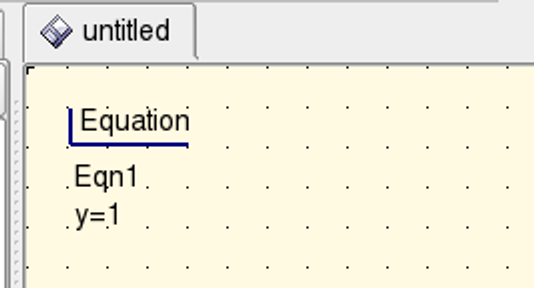
\includegraphics[%
  scale=0.4]{qucsformula2.png}\end{center}


\caption{\label{cap:Newly-created-equation}Newly created equation}
\end{figure}


You can now manipulate the current name of the equation
instance. Simply click onto {}``Eqn1'', which becomes
highlighted. Then type in a new name for it and finalise your inputs
with the <RETURN> key.

After that, you can enter a new equation. Again, click onto {}``y=1''.
Only the {}``1'' is marked, and you can enter a new expression there.
Please use the variables, operators and constants described in chapter
\textit{``\nameref{sec:Syntax}''}.  Note that you can also refer to
results (dependents) of other equations.  But how to change the name
of the current dependent {}``y''?  Right click onto the equation, and
a context menu opens.  Select the first item called {}``Edit
properties''.  A sub window appears, which should look like the one in
fig. \ref{cap:Editing-equation-properties}.  The alternative for
entering equations is to double click onto the equation.

%
\begin{figure}
\begin{center}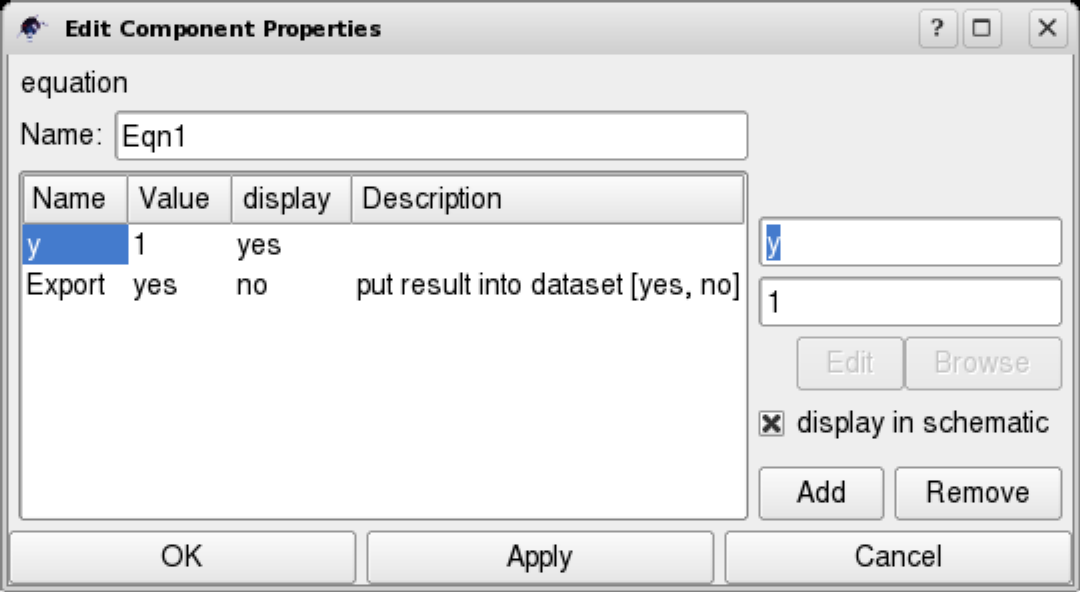
\includegraphics[%
  scale=0.4]{qucsformula3.png}\end{center}


\caption{\label{cap:Editing-equation-properties}Editing equation properties}
\end{figure}


You can now change the name of the dependent, the equation itself
(which is {}``1'' in the example shown) and the name of the equation.
If you do not want the result to be exported into the data display
tab, but temporarily need it for further calculations, select {}``no''
in the {}``Export value'' cell. 


\tutsubsection{\label{sec:Syntax}Syntax of Measurement Expressions}

Function names, variable names, and constant names are all case sensitive
in measurement expressions - it is distinguished between lowercase
and uppercase letters such as 'a' and 'A'.

In functions, commas are used to separate arguments.


\tutsubsubsection{Variable Names}

User defined variable names consist of a letter, followed by any number
of letters, digits, or underscores.

The syntax of variable names created by the \char`\"{}Qucs\char`\"{}
simulator is as specified in table~\ref{table:var_names}.  Please note
that all voltages and currents in {}``Qucs'' are peak values except
the noise voltages and currents which are rms values at 1Hz bandwidth.

%
\begin{table}[ht]
\begin{flushleft}\begin{tabular}{|r|l|}
\hline 
Variable Name&
Description\tabularnewline
\hline
\hline 
\textit{nodename}.V&
DC voltage at node \textit{nodename}\tabularnewline
\hline 
\textit{name}.I&
DC current through circuit component \textit{name}\tabularnewline
\hline 
\textit{nodename}.v&
AC voltage at node \textit{nodename}\tabularnewline
\hline 
\textit{name}.i&
AC current through circuit component \textit{name}\tabularnewline
\hline 
\textit{nodename}.vn&
AC noise voltage at node \textit{nodename}\tabularnewline
\hline 
\textit{name}.in&
AC noise current through circuit component \textit{name}\tabularnewline
\hline 
\textit{nodename}.Vt&
Transient voltage at node \textit{nodename}\tabularnewline
\hline 
\textit{name}.It&
Transient current through circuit component \textit{name}\tabularnewline
\hline
\textit{name}.OP&
\textit{name} = component name, OP = operating point (device dependent),\tabularnewline
&
 e.g. D1.Id\tabularnewline
\hline
S{[}x,y{]}&
S-parameter, e.g. S{[}1,1{]}\tabularnewline
\hline
Rn&
equivalent noise resistance\tabularnewline
\hline
Sopt&
optimal reflection coefficient for minimum noise\tabularnewline
\hline
Fmin&
minimum noise figure\tabularnewline
\hline
F &
noise figure\tabularnewline
\hline
\textit{nodename}.Vb&
Harmonic balance voltage at node \textit{nodename}\tabularnewline
\hline 
\end{tabular}\end{flushleft}


\caption{\label{table:var_names}Syntax of simulator generated variable names}
\end{table}



\tutsubsubsection{Numbers}

Numbers are written in conventional decimal way, with an optional
decimal point between the digits. For powers of ten, the familiar
scientific notation with an 'e' is used. In this way, '1.234e6' is an
example for the real floating point number 1234000. Imaginary numbers
can be entered by a multiplication factor 'i' or 'j' (see also table
\ref{table:constants}).  An example would be '1+2{*}i' or - if you
want to leave out the multiplication sign - '1+i2'.


\tutsubsubsection{Built-in constants}

The constants which can be used within measurement expressions are
given in table \ref{table:constants}.

%
\begin{table}[ht]
\begin{center}\begin{tabular}{|c|c|c|}
\hline 
Constant&
Description&
Value\tabularnewline
\hline
\hline 
e&
Euler's constant&
2.718282\tabularnewline
\hline 
i , j&
Imaginary unit $\left(\sqrt{-1}\,\right)$&
i1\tabularnewline
\hline 
kB&
Boltzmann's constant&
1.380658e23 J/K\tabularnewline
\hline 
pi&
$\pi$&
3.141593\tabularnewline
\hline
\end{tabular}\end{center}


\caption{\label{table:constants}Built-in Constants}
\end{table}



\tutsubsubsection{Operators}


\tutparagraph{Operator Precedence}

Expressions are evaluated in the standard way, meaning from left to
right, unless there are parentheses. The priority of operators is
also handled familiarly, thus for example multiplication has precedence
to addition. Table \ref{table:operators} specifies a sorted list
of all operators, the topmost having highest priority. Operators on
the same line have the same precedence.

%
\begin{table}[ht]
\begin{center}\begin{tabular}{|c|c|c|}
\hline 
Operator&
Name&
Example\tabularnewline
\hline
\hline 
()&
Parentheses, function call&
max(v)\tabularnewline
\hline 
\textasciicircum{}&
Exponentiation&
3\textasciicircum{}4\tabularnewline
\hline 
{*}&
Multiplication&
3{*}4\tabularnewline
/&
Division&
3/4\tabularnewline
\%&
Modulo&
4\%3\tabularnewline
\hline 
+&
Addition&
3+4\tabularnewline
-&
Subtraction&
3-4\tabularnewline
\hline 
:&
Range operator&
3:12\tabularnewline
\hline
\end{tabular}\end{center}


\caption{\label{table:operators}Operator priorities}
\end{table}



\tutparagraph{Ranges}

The general nomenclature of ranges is displayed in table \ref{table:Range-definition}.
It shows one-dimensional ranges, whereas also n-dimensional ranges
are possible, if you consider nested sweeps.

%
\begin{table}
\begin{center}\begin{tabular}{|c|c|}
\hline 
Syntax&
Explanation\tabularnewline
\hline
\hline 
m:n&
Range from index \textit{m} to index \textit{n}\tabularnewline
\hline 
:n&
Range up to index \textit{n}\tabularnewline
\hline 
m:&
Range starting from index \textit{m}\tabularnewline
\hline 
:&
No range limitations\tabularnewline
\hline
\end{tabular}\end{center}


\caption{\label{table:Range-definition}Range definition}
\end{table}



\tutsubsubsection{Post Processing of Simulation Data by Expressions}

After a simulation has run the results are stored in datasets. Usually,
such a dataset is a vector or a matrix, but may also be a real or
complex scalar. For transient analysis, this dataset contains voltage
or current information over time, for Harmonic Balance it contains
amplitudes at dedicated frequencies, while for S-parameter analysis
a vector of matrices (thus matrices in dependency of frequency) is
returned. In further generalisation the components of vectors and
matrices consist of complex numbers.

Additionally, datasets can be generated by using expressions. As an
example the linspace() function shall be named, which creates a vector
of linearly spaced elements.
